\documentclass{article}
\usepackage[utf8]{inputenc}
\usepackage{tikz}
\usepackage{amsmath}
\usetikzlibrary{positioning}

\begin{document}

%------------------------------------------------------------------------------
% QSPK
\begin{figure}[t]
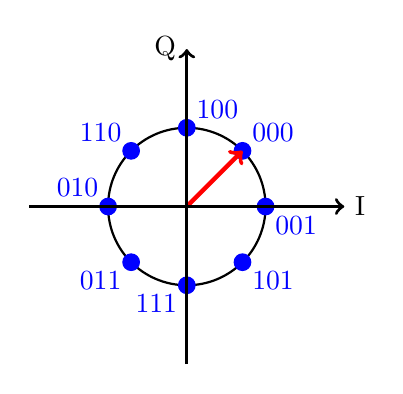
\begin{tikzpicture}
\draw[thick](0,0) circle (1);
\filldraw [blue] (1,0) circle (3pt) node[anchor=north west] {001};
\filldraw [blue] (0.707106781,0.707106781) circle (3pt) node[anchor=south west] {000};
\filldraw [blue] (0,1) circle (3pt) node[anchor=south west] {100};    
\filldraw [blue] (-0.707106781,0.707106781) circle (3pt) node[anchor=south east] {110};
\filldraw [blue] (-1,0) circle (3pt) node[anchor=south east] {010};  
\filldraw [blue] (-0.707106781,-0.707106781) circle (3pt) node[anchor=north east] {011};
\filldraw [blue] (0,-1) circle (3pt) node[anchor=north east] {111}; 
\filldraw [blue] (0.707106781,-0.707106781) circle (3pt) node[anchor=north west] {101};

\draw[red,ultra thick,->] (0,0) -- (0.707106781,0.707106781);

\draw[black,very thick,->] (-2,0) -- (2,0) node[anchor=west] {I};
\draw[black,very thick,->] (0,-2) -- (0,2) node[anchor=east] {Q};

\end{tikzpicture}
\end{figure}

\begin{equation*}
$X_k \in \cbrak{e^{j \frac{2\pi n}{8}}}   \quad n=0,1,\dots,7$
\end{equation*}
%------------------------------------------------------------------------------

\end{document}